%% Full length research paper template
%% Created by Simon Hengchen and Nilo Pedrazzini for the Journal of Open Humanities Data (https://openhumanitiesdata.metajnl.com)

\documentclass{article}
\usepackage[italian]{babel}
\usepackage[utf8]{inputenc}
\usepackage{johd}
\usepackage{graphicx}
\usepackage{graphics}
\documentclass{article}
\usepackage{listings}
\usepackage{color}

\title{Relazione - Confronto tra combinazioni di coppie microfoniche per la registrazione di un organo}

\author{Gabriele Acquafredda$^{a}$$^{*}$ \\
    \small $^{a}$2° Anno di Tecnica Del Suono, Primo livello, Dipartimento di Musica Elettronica\\
    \small  Conservatorio di Musica Niccolò Piccinni, Bari, Italia\\
}

\date{Novembre 2022} 

\begin{document}

\maketitle

\begin{abstract} 
    \noindent La presente relazione vuole studiare le differenze in termini di resa sonora e stereofonia di diverse combinazioni di microfoni per la registrazione di un organo, valutando analiticamente una moltitudine di parametri. La motivazione principale della relazione-ricerca non è fornire un dato oggettivo di quale delle combinazioni risulta essere migliore - anche se all'atto pratico c'è una preferita, ma il gusto non è parte della relazione - quanto valutare le differenze e stabilire le discriminanti che ci possano dare la possibilità di scegliere una combinazione piuttosto che un'altra nei differenti contesti di registrazione, così come cercare dei modi per sfruttare al meglio ciascuna delle configurazioni in post-produzione.
\end{abstract}

\section{Informazioni Preliminari}

Le registrazioni sono state effettuate nell'ambito del premio nazionale delle arti del 2022 con l'aiuto dei corsisti del Dipartimento di Musica Elettronica del Conservatorio di Bari con l'aiuto del maestro Silvi Giuseppe. 

\subsection{L'organo}

    Per parlare dell'organo è necessario calarlo nel contesto: l'organo, difatti, è parte integrante dell'auditorium del conservatorio. Questa è un'importante informazione che ci suggerisce anche il come sono state affrontate le registrazioni dei brani. Il fine ultimo del lavoro non è stato, difatti, una mera registrazione dell'organo, ma dell'organo che risuona nel suo stesso spazio. 
    \begin{figure}[H]
        \centering
        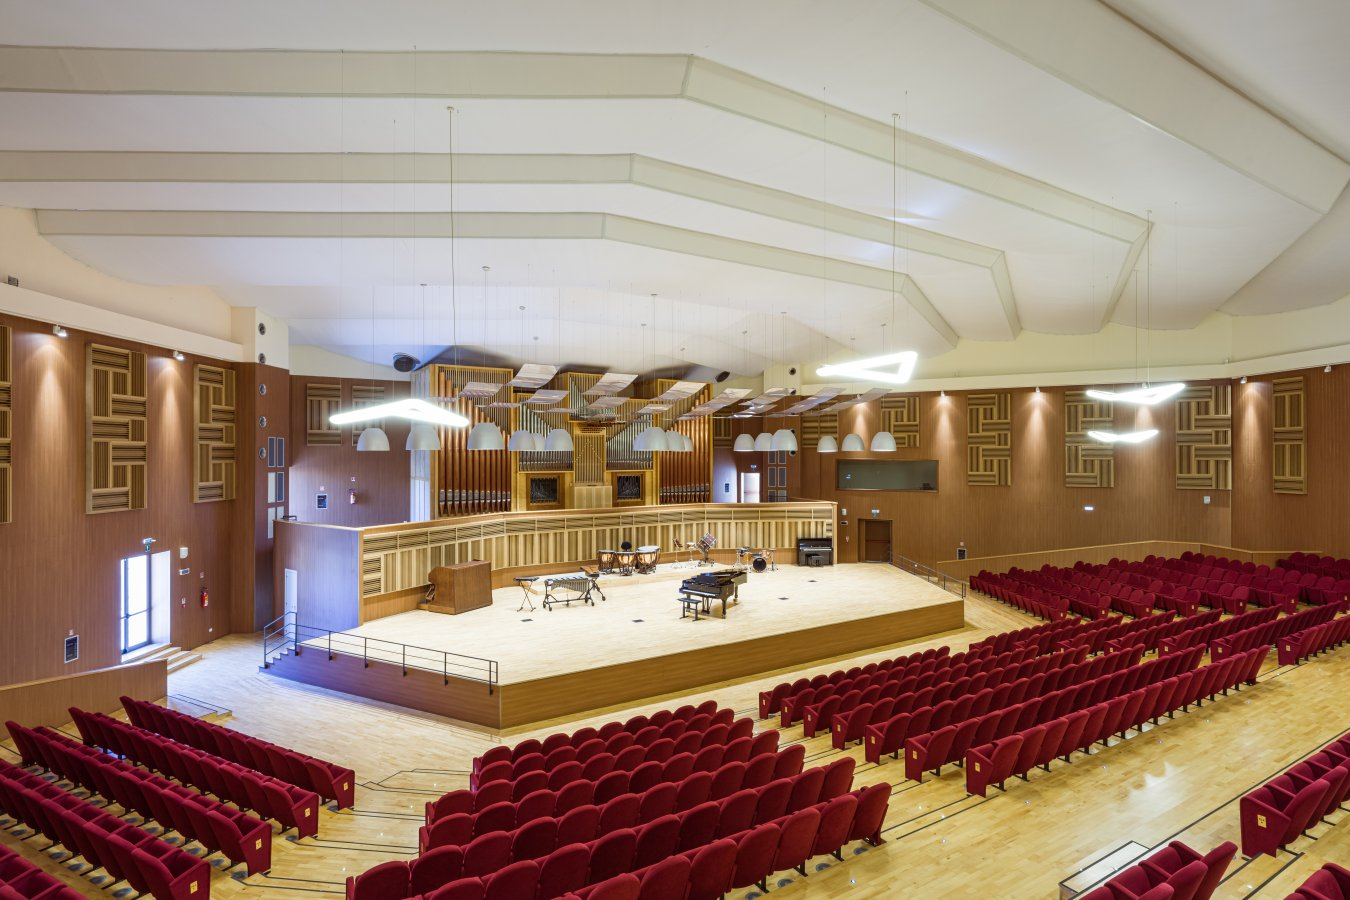
\includegraphics[width=0.5\textwidth]{images/auditorium-organo.jpg}
        \caption{\label{fig1}L'organo dell'auditorium Nino Rota.}
    \end{figure}
    \noindent L'organo è stato costruito nel 1980 dalla ditta Tamburini di Crema, nota per la costruzione degli strumenti del Duomo di Milano e della Basilica di San Pietro a Roma. È alto 7 metri e largo 12, contando circa 5000 canne, tre tastiere, una pedaliera e ben 75 timbri sonori.
    L'auditorium è di pianta esagonale con 3000 mq di superficie e 500 posti a sedere. 
\endsubsection


\subsection{Descrizione analitica della strumentazione adoperata}

Per le registrazioni è stata adoperata la seguente strumentazione:
\begin{itemize}
    \item[A.] N.2 Microfoni LINE AUDIO CM4
    \item[B.] N.4 Microfoni LINE AUDIO OM1
    \item[C.] N.1 Microfono Schoeps MSTC 74 (Stereo/ORTF)
    \item[D.] N.1 Mixer Allen Heath SQ5
    \item[E.] Cavi Cordial
\end{itemize}


\subsubsection{A. Specifiche tecniche LINE AUDIO CM4}
    \begin{figure}[H]
        \centering
        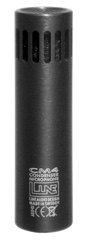
\includegraphics[width=0.1\textwidth]{images/CM4.jpg}
        \caption{\label{fig2}LINE AUDIO CM4.}
    \end{figure}
    
    Il LINE AUDIO CM4 è un microfono una risposta in frequenza particolarmente piatta in relazione al suo costo. È molto adatto alle situazioni dove è necessaria resa sonora particolarmente fedele a quello che è il materiale da registrare - come ad esempio nelle registrazioni di musica strumentale e classica. Qui le informazioni più rilevanti per il nostro lavoro di regitrazione.\\\\
    Tipologia: Microfono a Condensatore - necessita phantom a 48 V. \\
    Figura Polare: Cardioide (leggermente più ampio)\\
    Risposta in frequenza: 20 Hz - 20kHz\\
    Rapporto Segnale/Rumore: 78dB/68dB\\
    Noise Level: 16 dB(A)\\
    Max SPL: 140 dB
    
    \begin{figure}[H]
        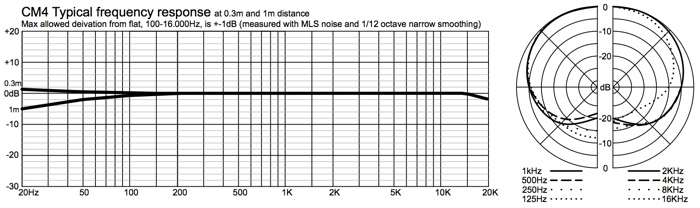
\includegraphics[width=1\textwidth]{images/CM4PLOT.jpg}
        \caption{\label{fig3}Risposta in frequenza e polar pattern LINE AUDIO CM4.}
    \end{figure}
\endsubsubsection

\subsubsection{B. Specifiche tecniche LINE AUDIO OM1}
    \begin{figure}[H]
        \centering
        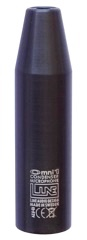
\includegraphics[width=0.1\textwidth]{images/Omni1.jpg}
        \caption{\label{fig4}LINE AUDIO OM1.}
    \end{figure}
    
    Il LINE AUDIO OM1 è l'analogo omnidirezionale del CM4.\\\\
    Tipologia: Microfono a Condensatore - necessita phantom a 48 V. \\
    Figura Polare: Omnidirezionale (dai 16Khz si schiaccia diventando quasi subcardioide)\\
    Risposta in frequenza: 20 Hz - 20kHz\\
    Rapporto Segnale/Rumore: 76dB/66dB\\
    Noise Level: 18 dB(A)\\
    Max SPL: 133 dB
    
    \begin{figure}[H]
        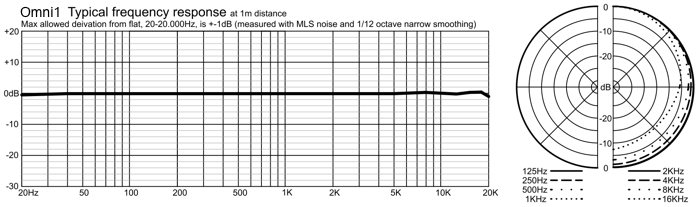
\includegraphics[width=1\textwidth]{images/Omni1plot.png}
        \caption{\label{fig5}Risposta in frequenza e polar pattern LINE AUDIO OM1.}
    \end{figure}
\endsubsubsection

\subsubsection{C. Specifiche tecniche Schoeps MSTC 74}
    \begin{figure}[H]
        \centering
        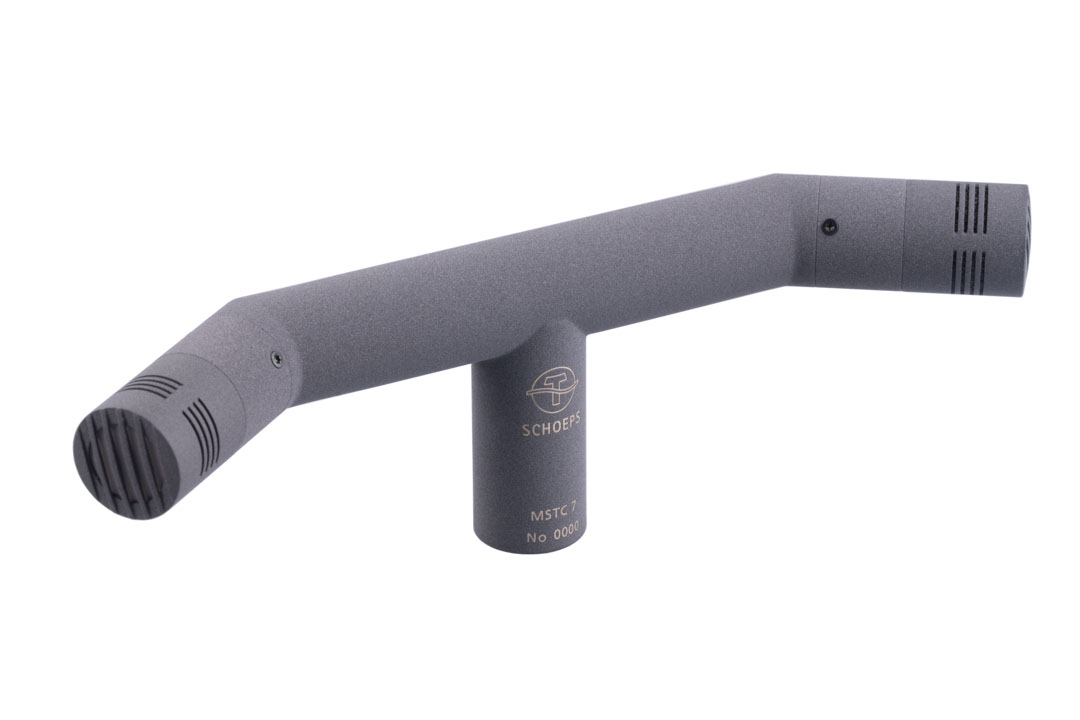
\includegraphics[width=0.4\textwidth]{images/MSTC74.jpeg}
        \caption{\label{fig6}Lo Schoeps MSTC 74.}
    \end{figure}
    
    Questo microfono Schoeps viene spesso adoperato come coppia main per la registrazione di ensemble, cori o come semplice microfono stereo. Consiste in una caratteristica forma a T con due capsule Schoeps MK4 distanziate a 170 mm con un'angolatura di 110° - caratteristiche tipiche della microfonazione ORTF\\\\
    Tipologia: Microfono a Condensatore - necessita phantom a 48 V.\\
    Figura Polare di ciascuna capsula MK4: Cardioide (con la tendenza a deformarsi dagli 8kHz in poi)\\
    Risposta in frequenza: 40 Hz - 26kHz\\
    Rapporto Segnale/Rumore: 80dB\\
    Noise Level: 14 dB(A)\\
    Max SPL: 135 dB
    
    \begin{figure}[H]
        \centering
        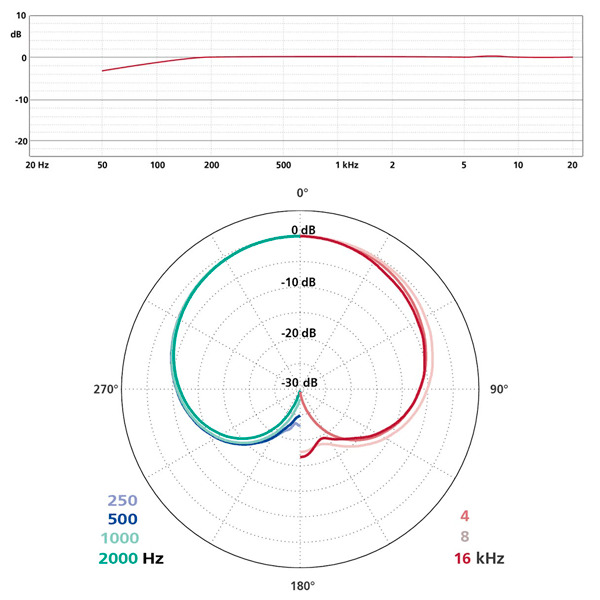
\includegraphics[width=0.5\textwidth]{images/PLOT_SCHOEPS.jpg}
        \caption{\label{fig7}Risposta in frequenza e polar pattern di ciascuna capsula MK4 dello Schoeps MSTC 74.}
    \end{figure}
\endsubsubsection

\subsubsection{D. Descrizione e Configurazione Allen Heath SQ5}
    \begin{figure}[H]
        \centering
        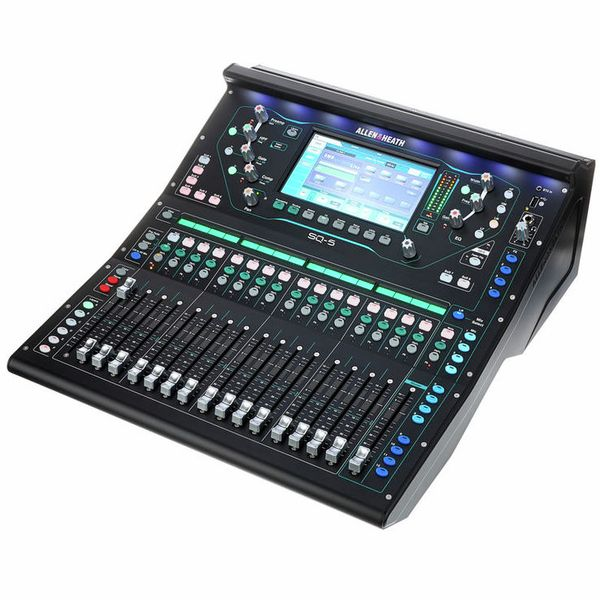
\includegraphics[width=0.4\textwidth]{images/SQ5.jpg}
        \caption{\label{fig7}L'Allen Heath SQ5.}
    \end{figure}
    
    L'Allen Heath SQ5 è un mixer digitale a 48 canali. Il mixer per le registrazioni è stato impostato per funzionare ad una frequenza di campionamento di 96KHz e 24 bit di profondità.
    La configurazione dei canali è stata:
    \begin{itemize}
        \item[1.] ORTF-L
        \item[2.] ORTF-R
        \item[3.] AB-L
        \item[4.] AB-R
        \item[5.] STOSS1
        \item[6.] STOSS2
        \item[7.] STOSS3
        \item[8.] STOSS4
        \item[9.] SOUNDFIELD-W
        \item[10.] SOUNDFIELD-X
        \item[11.] SOUNDFIELD-Y
        \item[12.] SOUNDFIELD-Z
        \item[13.] FAULKNER-NOS-L
        \item[14.] FAULKNER-NOS-R
        \item[15.] FAULKNER-FLANK-L
        \item[16.] FAULKNER-FLANK-R
    \end{itemize}
\endsubsubsection
\endsubsection

\section{Schema di posizionamento delle configurazioni microfoniche}
    \begin{figure}[H]
        \centering
        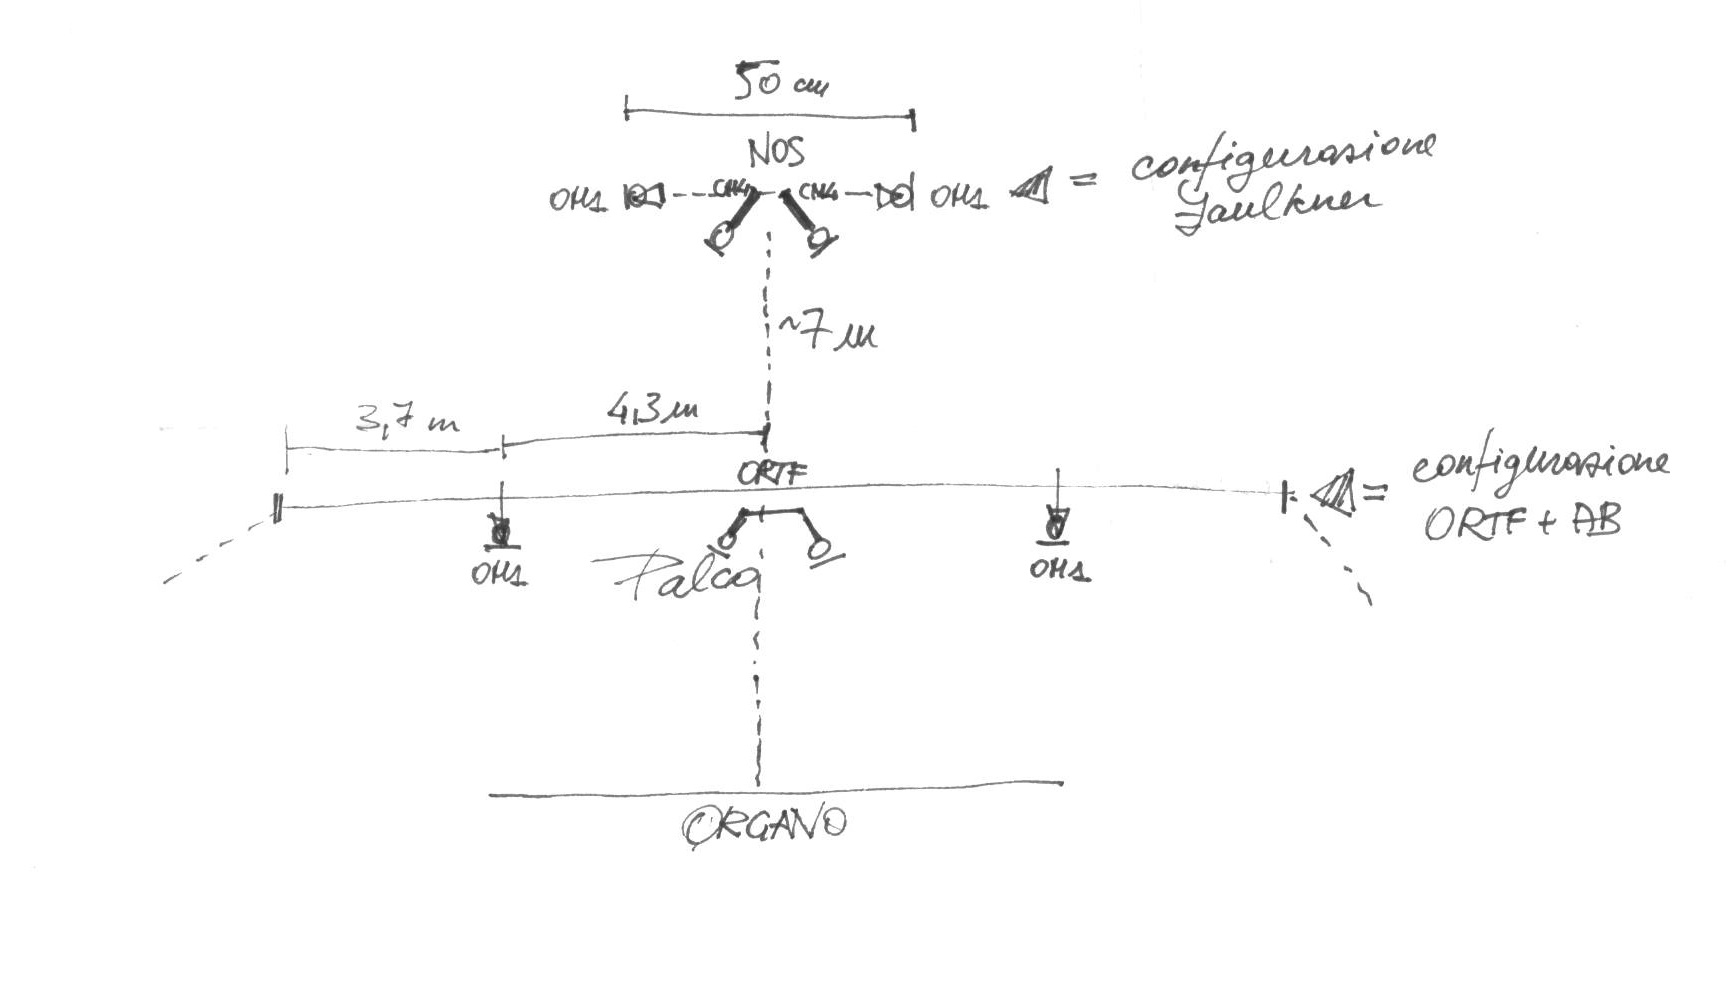
\includegraphics[width=1\textwidth]{images/schema.jpg}
        \caption{\label{fig8}Configurazioni microfoniche}
    \end{figure}
    
    Le due configurazioni oggetto di analisi sono una classica ORTF+AB ed un Faulkner Array "compresso".
    La prima configurazione ORTF+AB è stata posizionata al ciglio del palco, la seconda a circa 7 metri dal palco.
    
    \subsection{Descrizione Prima Configurazione}
        La prima configurazione ORTF+AB è da considerarsi come una combinazione di coppie stereofoniche che ci permettono di bilanciare il Mid ed il Side delle registrazioni. L'ORTF, configurazione che consiste in una coppia di microfoni posizionati tra di loro a 110° e con una distanza tra le capsule di 17 cm. Questa combinazione stereo ci è utile come mid. In confronto all'organo, difatti, l'ORTF, seppur una coppia stereofonica discretamente ampia, ci da un'informazione particolarmente "ristretta" dell'immagine stereo, che ci aiuta a rinforzare le informazioni del "side microfonico", costituito dalla coppia AB di 2 OM1.
    
        \begin{figure}[H]
            \centering
            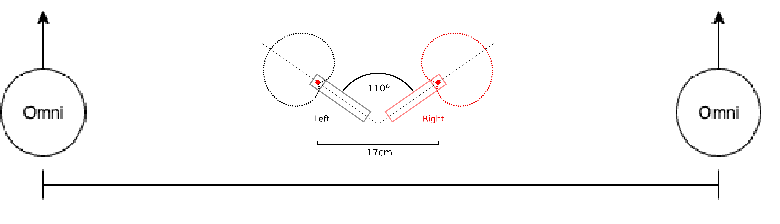
\includegraphics[width=0.8\textwidth]{images/ortfab.png}
            \caption{\label{fig9}Configurazione ORTF+AB}
        \end{figure}
    \endsubsection
        
    \subsection{Descrizione Seconda Configurazione}    
        La seconda configurazione è un Faulkner array. Esso è costituito da una combinazione di una coppia NOS fatta con due CM4 ed una coppia AB fatta con due OM1. Analogamente alla prima configurazione, avremo un'informazione con una immagine stereo ristretta nella coppia di CM4 e una allargata da parte dei due OM1. Questa configurazione, a differenza dell'altra, è più distante dal palco e - ovviamente - produrrà dei risultati molto differenti nell'analisi.
    \endsubsection
\endsection 

\section{Analisi delle due configurazioni}
    \subsection{Prime Considerazioni}
    A registrazione conclusa, i risultati sono stati molto differenti per le due configurazioni.
    Qui un plot dello spettrogramma e dello stereo field analyzer per le due configurazioni in uno stesso punto.
    
    \begin{figure}[H]
        \centering
        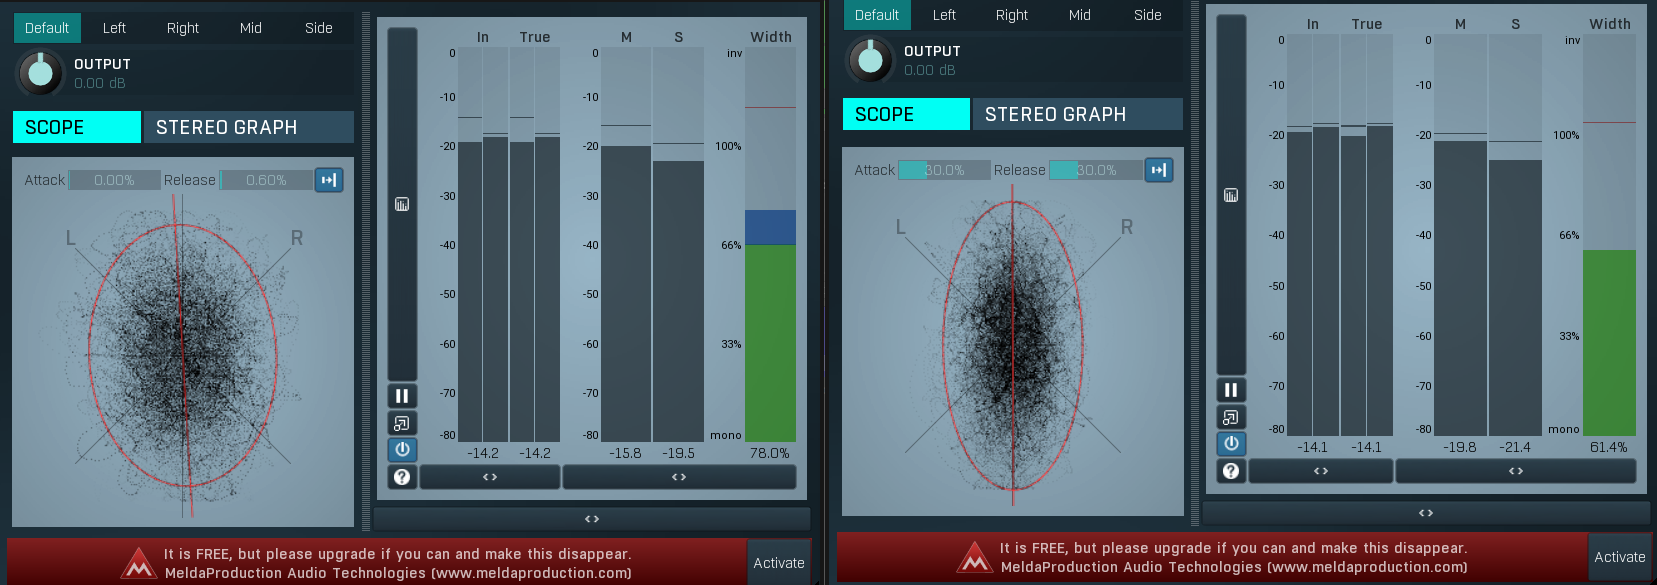
\includegraphics[width=1\textwidth]{images/1PLOT-STEREOSCOPE.png}
         \caption{\label{fig10}A sx - ORTF+AB | A dx - FAULKNER ARRAY}
    \end{figure}
    
    \begin{figure}[H]
        \centering
        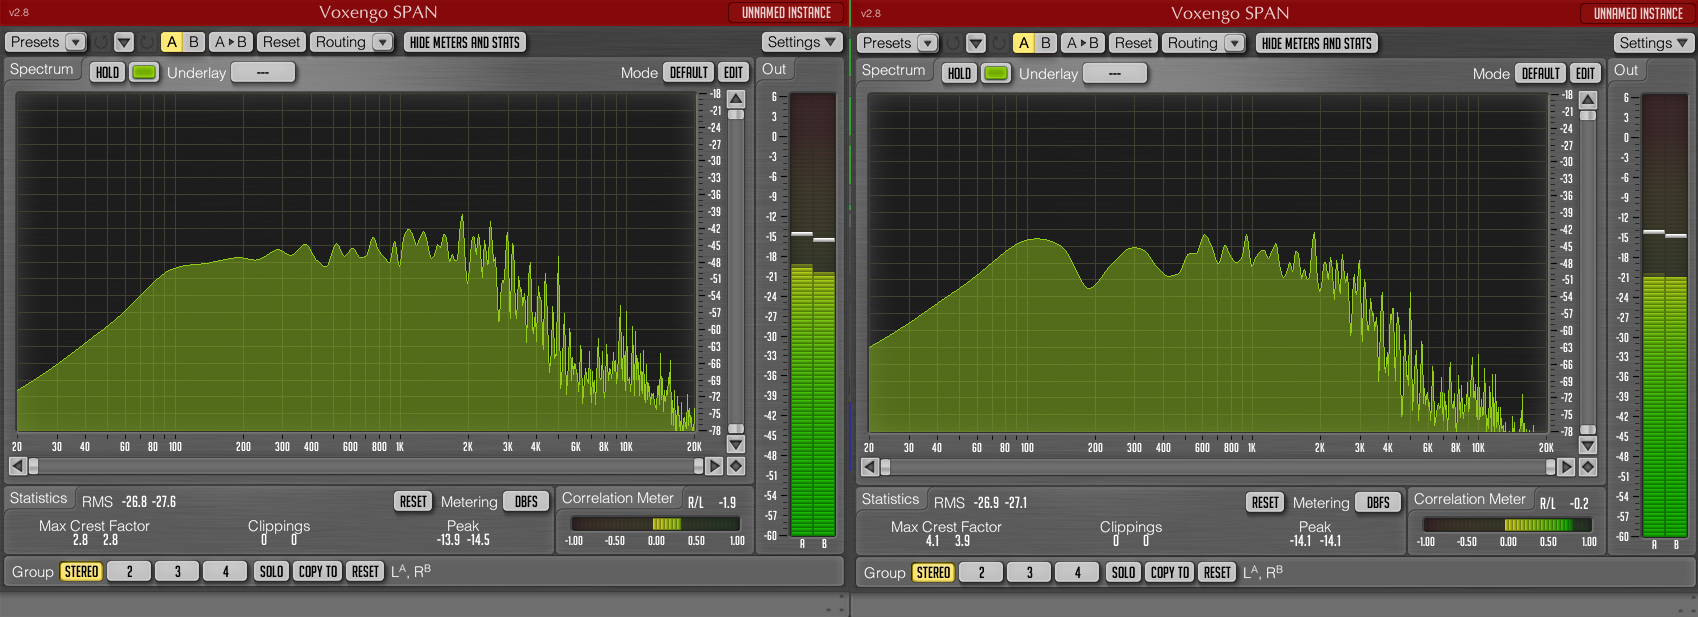
\includegraphics[width=1\textwidth]{images/1PLOT-SPAN.png}
         \caption{\label{fig11}A sx - ORTF+AB | A dx - FAULKNER ARRAY}
    \end{figure}
    
    \begin{itemize}
        \item A primo acchito abbiamo rilevato che la coppia del frontepalco era decisamente troppo vicina all'organo, dandoci una risposta molto brillante dei registri frontali dell'organo ed una molto più affievolita dei registri più gravi.
        \item La seconda configurazione più lontana, invece, ha subito il problema opposto: una ottima risposta delle basse, ma delle alte più confuse, soprattutto per via della distanza dai registri acuti e per la riverberazione dello spazio acustico.
        \item Come rilevato dal plot dell'MStereoScope, la seconda configurazione, a differenza della prima, ci da un'informazione stereofonica molto più ristretta. Nello stesso punto (un fortissimo dell'organo), abbiamo nel frontepalco una "width" del 75\% circa, invece nella seconda configurazione abbiamo circa il 60\%
        \item Nei passaggi più veloci del brano suonato, la prima configurazione è decisamente più nitida e piacevole all'ascolto. Nella seconda lo spazio riverberante si rende complice di una resa sonora decisamente più confusionaria che fa perdere il senso melodico del brano in favore di quello prettamente armonico. Ne consegue che sui passaggi più lenti, la seconda configurazione è più ricca, seppur offra generalmente meno dettaglio
        \item Le due configurazioni, quindi, differiscono l'una per il dettaglio della stanza, l'altra per il dettaglio dello stesso organo.
    \end{itemize}
\endsubsection
    
\subsection{Analisi delle frequenze basse}
    Come già accennato, le frequenze basse rispondono diversamente nelle due configurazioni. Ci è utile quindi ispezionarle nel dettaglio. Per fare questo, ci avvaliamo del preset "Lo-Freq inspection" dell'analizzatore Voxengo SPAN. Il punto del brano in cui viene effettuata l'analisi è lo stesso dell'analisi precedente.
    
    \begin{figure}[H]
        \centering
        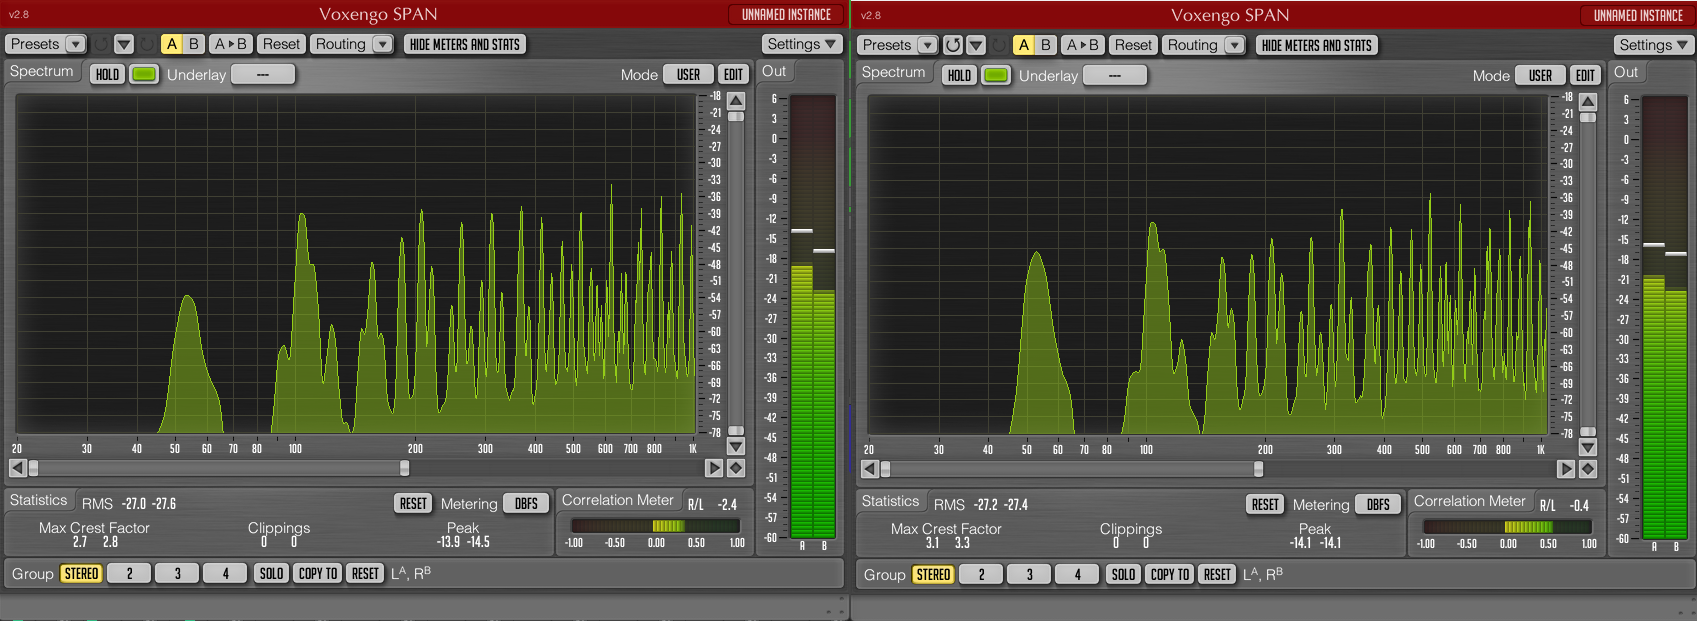
\includegraphics[width=1\textwidth]{images/2PLOT-SPAN.png}
         \caption{\label{fig11}A sx - ORTF+AB | A dx - FAULKNER ARRAY}
    \end{figure}
    
    Come ben dimostrato dall'analisi, il contenuto di basse delle due configurazioni è molto diverso. Abbiamo infatti una miglior risposta nella seconda configurazione. La spiegazione di questo fenomeno è che le frequenze basse, data la lunghezza d'onda ben più ampia delle altre frequenze (che a 50 Hz è circa di 6,4 m), hanno la necessità di avere più spazio per svilupparsi, ma non solo: c'è da considerare anche il fatto che le canne dell'organo che riproducono i suoni più bassi sono rivolte verso l'alto. Conseguentemente ad una distanza maggiore, abbiamo una migliore risposta in registrazione di queste canne, riuscendo a dare "l'aria" giusta per il loro sviluppo e la loro ripresa.
\endsubsection 

\subsection{Esperimento - Variazione della risposta stereofonica al variare dell'ampiezza delle singole coppie}
    Per valutare la versatilità delle coppie e la loro risposta nel bilanciamento del mid/side, un buon metodo potrebbe essere quello di vedere qual è la differenza in termini di immagine stereo e nel contenuto frequenziale al variare dell'ampiezza della coppia main e della coppia flank di entrambe le configurazioni.
    Come primo esperimento, settiamo il fader dei flank di entrambe le coppie a -6 dB, in modo da fare una prima analisi. Il risultato è il seguente:
    
    \begin{figure}[H]
        \centering
        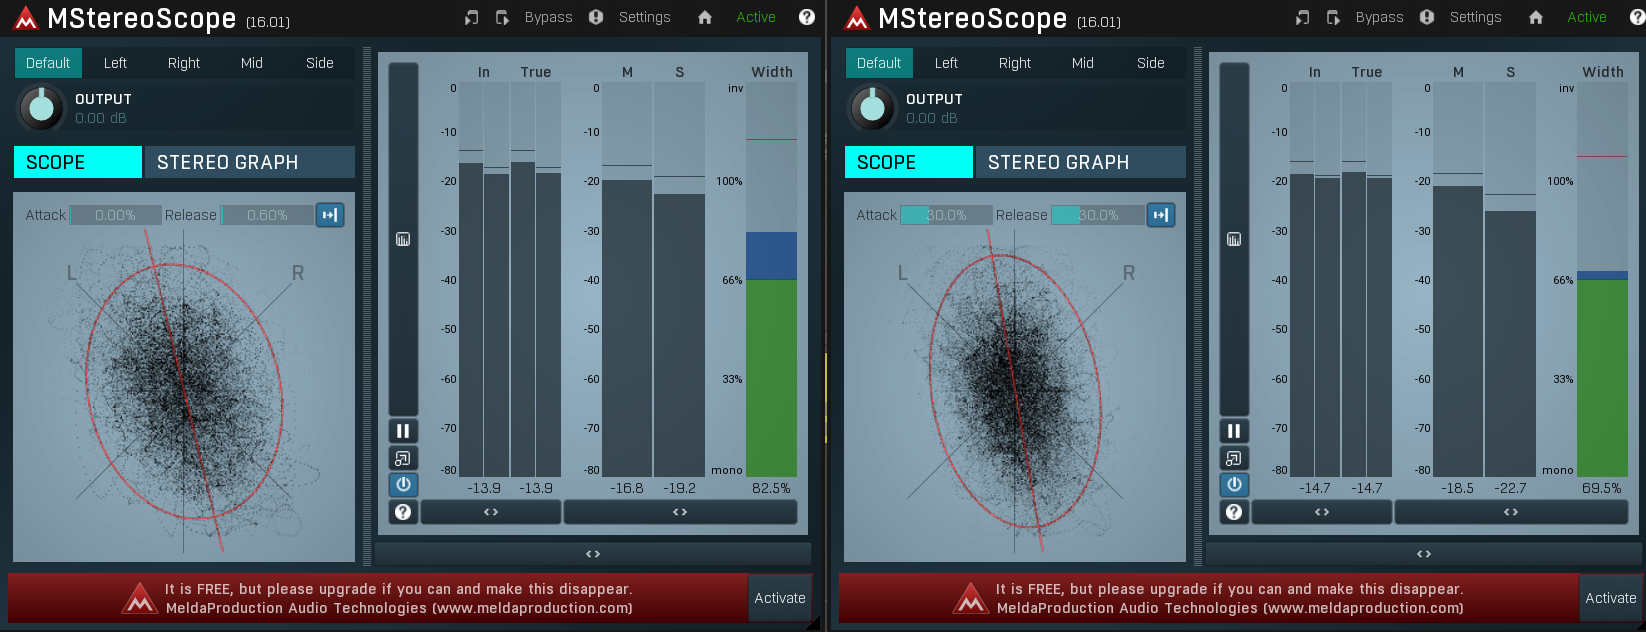
\includegraphics[width=1\textwidth]{images/3PLOT-6AB-STEREOSCOPE-FRONTEPALCO.png}
         \caption{\label{fig11}A sx - ORTF+AB normale | A dx - ORTF con AB a -6 dB}
    \end{figure}
    
    \begin{figure}[H]
        \centering
        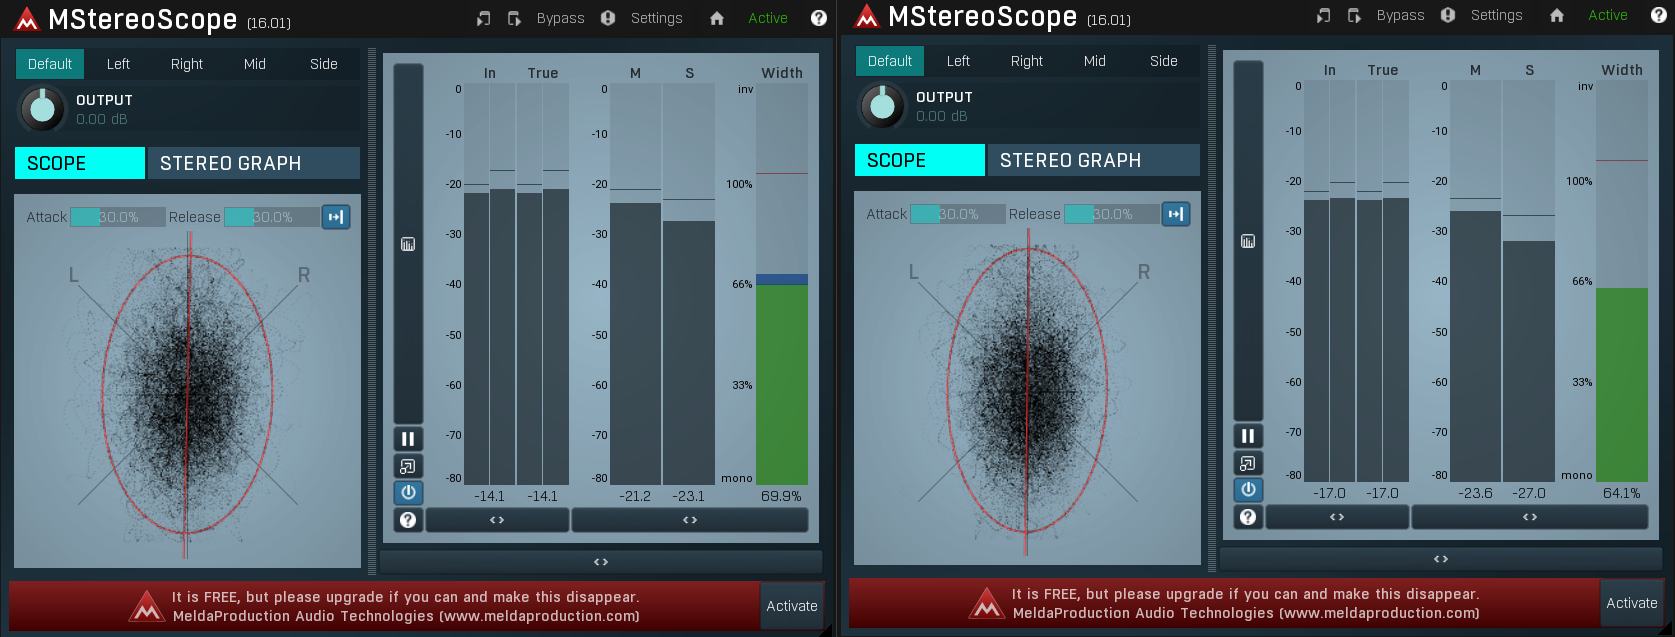
\includegraphics[width=1\textwidth]{images/3PLOT-6AB-STEREOSCOPE-FAULKNER.png}
         \caption{\label{fig11}A sx - Faulkner normale | A dx - Faulkner con AB a -6 dB}
    \end{figure}
    
    Il risultato non ci sorprende più di tanto: rileviamo che nella prima configurazione, una differenza d'ampiezza della coppia AB incide in maniera cruciale sulla qualità dell'immagine stereofonica, dandoci un minore dettaglio anche della "grandezza" dell'organo. Nella seconda configurazione, invece, non vi è un'enorme differenza in termini di stereo width tra i 0 e -6 dB dell'AB. Questo risultato era quasi ovvio sin dall'inizio poiché la prima coppia AB è molto più spaziata della seconda. Conseguentemente nella seconda configurazione, la coppia AB non risulta sufficientemente utile in termini di dettaglio stereofonico. Sarebbe stato più utile, eventualmente, spaziare ulteriormente i due flank, in modo da ottenere un risultato più dettagliato e meno confusionario.
    A riconferma di questo, possiamo prendere in analisi le AB di ciascuna delle due configurazioni:
    
    \begin{figure}[H]
        \centering
        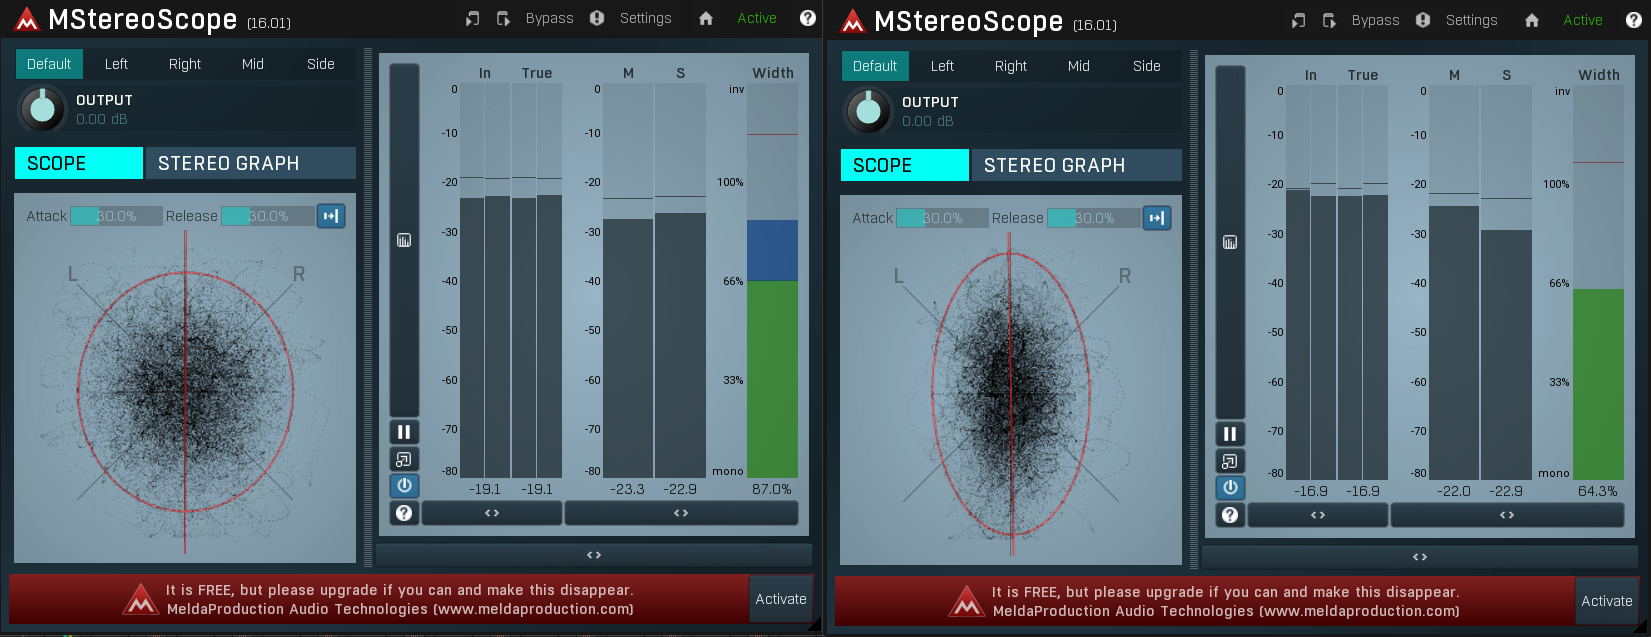
\includegraphics[width=1\textwidth]{images/4PLOT-AB.png}
         \caption{\label{fig11}A sx - AB del frontepalco | A dx - AB del Faulkner}
    \end{figure}
    
    La differenza tra le due coppie AB è schiacciante ed è palesemente udibile. Si passa da un'apertura estrema e quasi sguaiata del frontepalco, dove la correlazione tra sinistra è destra è quasi nulla, ad un campo ristretto dato dalla coppia AB del Faulkner Array.
    Diversa è la situazione tra le due coppie main delle due configurazioni, che in termini di informazioni stereofoniche, sono pressoché uguali, ma con un contenuto frequenziale decisamente diverso.
    
    \begin{figure}[H]
        \centering
        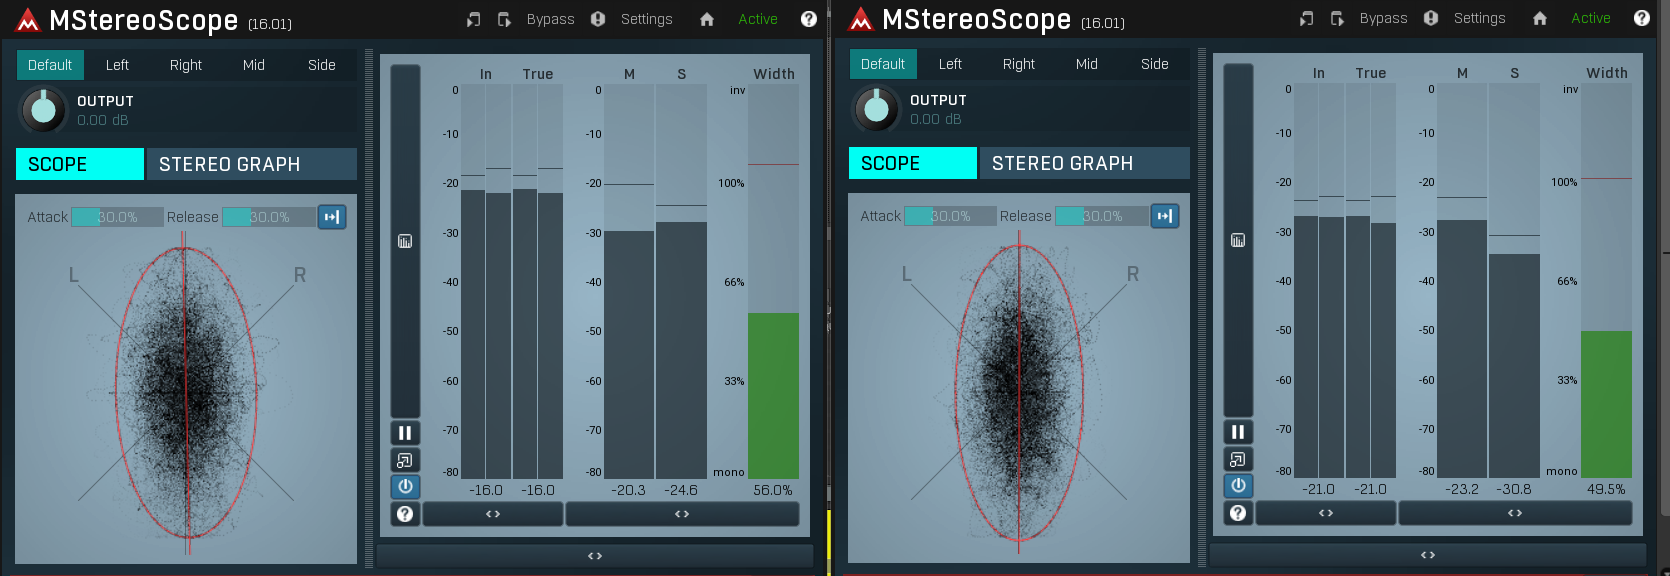
\includegraphics[width=1\textwidth]{images/4PLOT-MAIN.png}
         \caption{\label{fig11}A sx - Main del frontepalco | A dx - Main del Faulkner}
    \end{figure}
\endsubsection

\subsection{Esperimento - Analisi Mid/Side con una matrice somma/differenza}
    Una matrice somma differenza è capace di fare solo calcoli matematici sui segnali: nel nostro caso farà L+R ed L-R, che per definizione sono rispettivamente mid e side. Analizzare separatamente mid e side, ci aiuta a capire quante informazioni abbiamo "al centro" e quante "ai lati" di ciascuna coppia microfonica e di ciascuna configurazione.
    Come prima cosa, dovremmo costruire un encoder/decoder mid/side. Per far questo ci serviamo di Faust e costruiamo un plugin apposta.
    
    \lstset{frame=tb,
          language=c++,
          aboveskip=5mm,
          belowskip=5mm,
          showstringspaces=false,
          columns=flexible,
          basicstyle={\small\ttfamily},
          numbers=none,
          numberstyle=\tiny\color{blue},
          keywordstyle=\color{red},
          commentstyle=\color{pink},
          stringstyle=\color{green},
          breaklines=true,
          breakatwhitespace=true,
          tabsize=3}
          
    \begin{lstlisting}
        import("stdfaust.lib"); //LIBRERIA STANDARD
        nsum = + / sqrt(2);
        ndiff = - / sqrt(2);
        sdmx =  _, _ <: nsum, ndiff; //MAIN
        process = sdmx(_,_);
    \end{lstlisting}
    
    Nel risultato troveremo la somma - quindi il mid - nel primo canale, la differenza - quindi il side - nel secondo canale.
    Servendoci di questo strumento, analizziamo per ciascuna configurazione il mid ed il side:
    
    \begin{figure}[H]
        \centering
        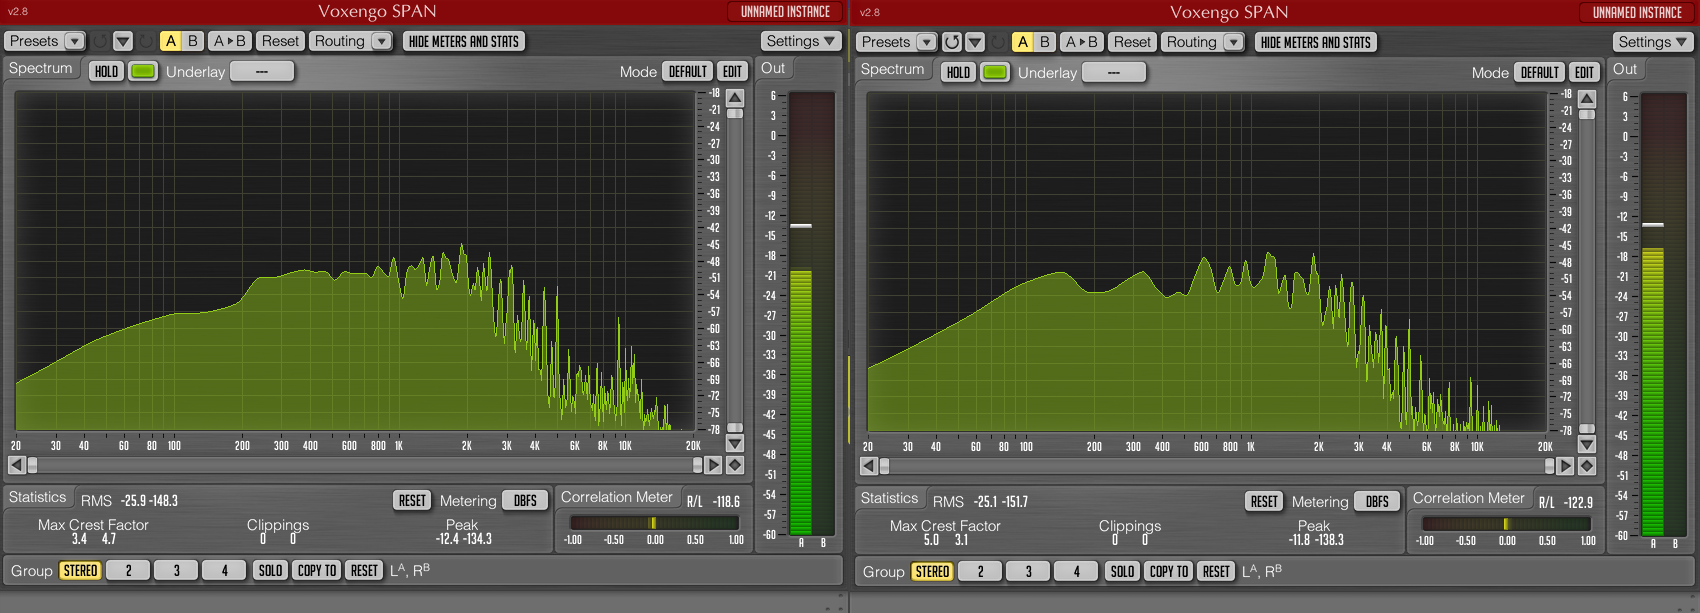
\includegraphics[width=1\textwidth]{images/5PLOT-MID.png}
         \caption{\label{fig11}A sx - MID del frontepalco | A dx - MID del Faulkner}
    \end{figure}
    
    \begin{figure}[H]
        \centering
        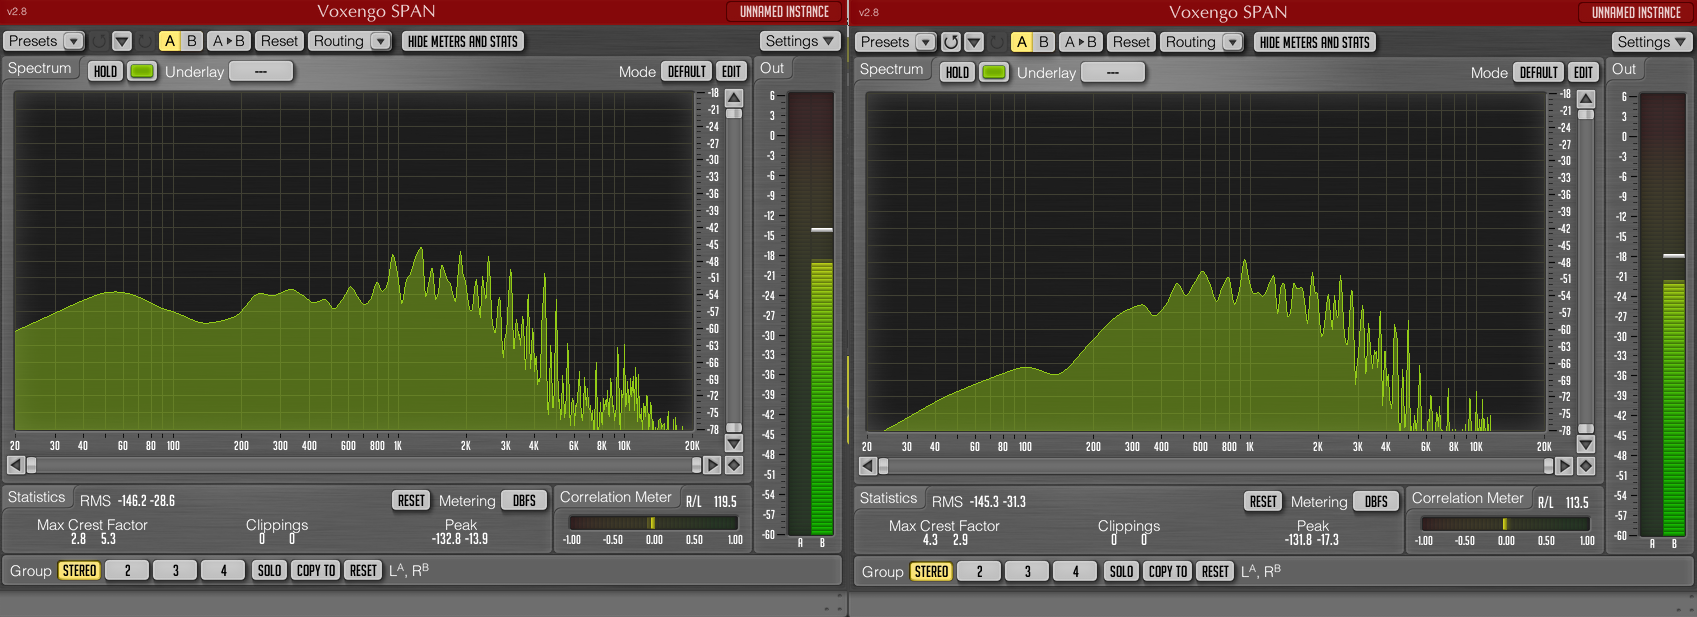
\includegraphics[width=1\textwidth]{images/5PLOT-SIDE.png}
         \caption{\label{fig11}A sx - SIDE del frontepalco | A dx - SIDE del Faulkner}
    \end{figure}
    
    I risultati di questa analisi sono molto interessanti: notiamo una maggiore risposta sulle basse nel mid del faulkner. La situazione si inverte - sorprendentemente - invece, nel side del frontepalco. La maggior parte delle informazioni delle basse, quindi, la abbiamo nel side piuttosto che nel mid considerando la configurazione frontepalco. La seconda configurazione, invece, ci da un risultato più "convenzionale" e forse anche più corretto: abbiamo una migliore risposta delle basse sul mid, e molte meno basse sul side.
    Nelle alte viene ripuntualizzata una carenza nella configurazione Faulkner rispetto al frontepalco, sia considerando il mid, che il side.
    A livello di resa sonora, il mid della configurazione Faulkner risulta piuttosto confuso ed impastato anche se "formalmente più corretto" rispetto al mid del frontepalco - ciò ci suggerisce che l'utilizzo improprio ed esclusivo degli analizzatori di spettro piuttosto che l'utilizzo di un orecchio critico, ci può dare risultati formalmente corretti, ma percettivamente disastrosi. Il mid del frontepalco, però, risulta comunque più "sgonfio" rispetto a quello della configurazione Faulkner, ma decisamente più definito nei particolari.
    Il side della configurazione Faulkner invece, seppur oggettivamente meno incisivo ed alto di volume rispetto a quello del frontepalco (cosa evidente già dal precedente esperimento), contiene una maggiore informazione su quella che è la dimensione dell'auditorium. Nel side invece del frontepalco abbiamo più informazioni dirette dell'organo che, per quanto piacevoli, vanno a snaturare il suono dell'organo, scorporandolo dal suo stesso ambiente.
    
\subsection{Esperimento - E se usassimo i flank come side e il main come mid?}
    Un esperimento molto particolare potrebbe essere quello di usare, in ciascuna configurazione, il mid della coppia main e combinarlo col side della coppia flank. Questo esperimento potrebbe avere senso in quanto usiamo al centro le informazioni provenienti fisicamente dal centro, e ai lati le informazioni captate fisicamente ai lati.
    I risultati di questo esperimento sono molto interessanti:
    
    \begin{figure}[H]
        \centering
        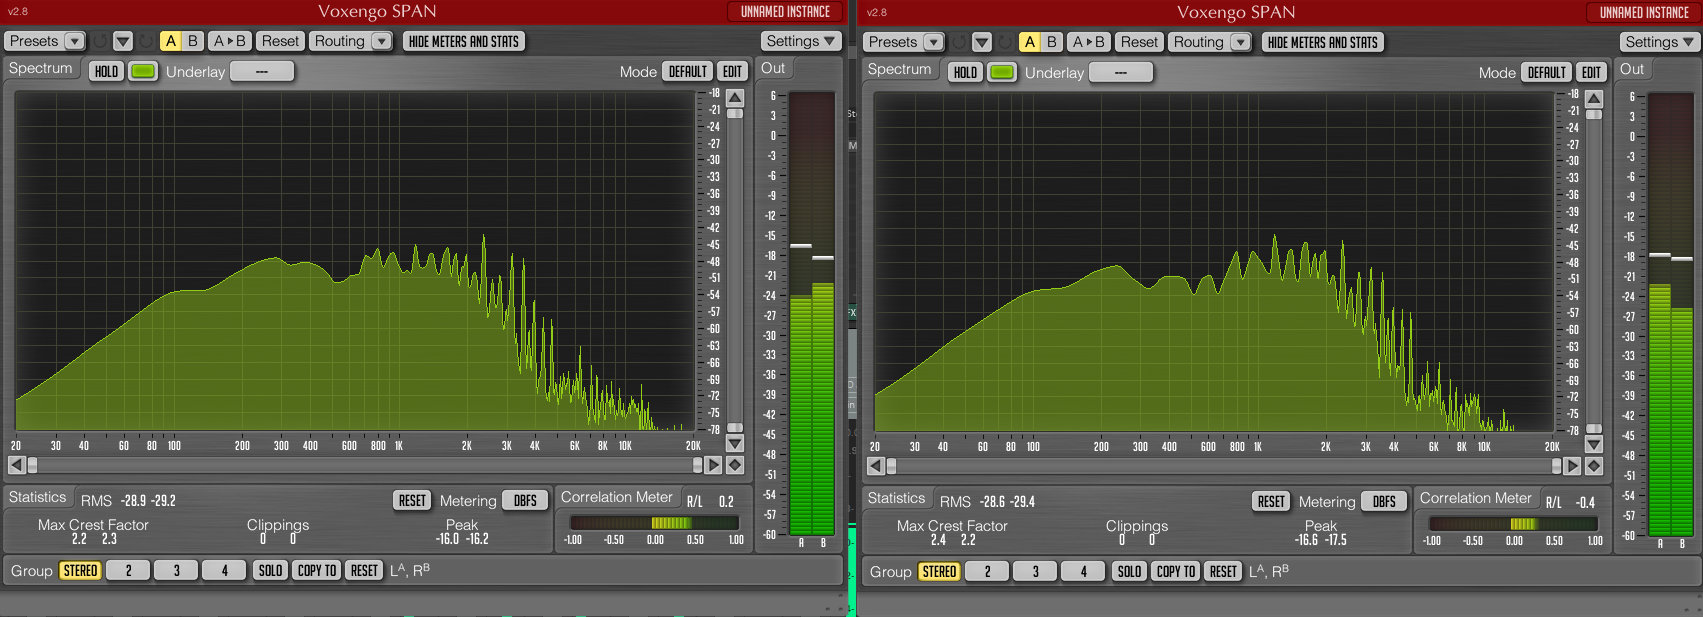
\includegraphics[width=1\textwidth]{images/6PLOT-MID-SIDE.png}
         \caption{\label{fig11}A sx - L'esperimento sul frontepalco | A dx - L'esperimento sul Faulkner}
    \end{figure}
    
    \begin{figure}[H]
        \centering
        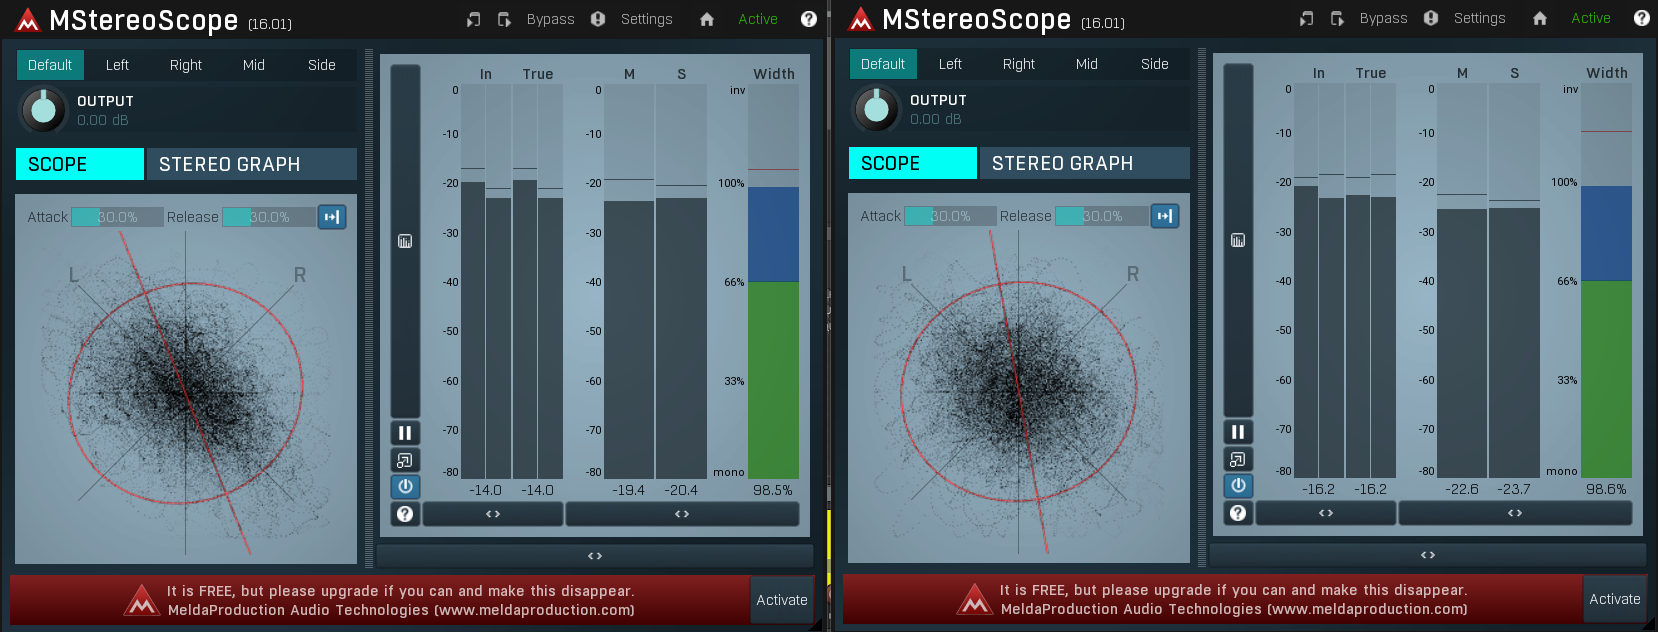
\includegraphics[width=1\textwidth]{images/6PLOT-MID-SIDE-STEREO.png}
         \caption{\label{fig11}A sx - L'esperimento sul frontepalco | A dx - L'esperimento sul Faulkner}
    \end{figure}
    
    Graficamente abbiamo dei risultati molto simili, all'orecchio anche, se non per un particolare già citato: la percezione dell'ambiente della configurazione frontepalco ci da una maggiore resa della fonte diretta a scapito della riflessa. Però è molto interessante analizzare come i risultati siano molto simili tra le due configurazioni. C'è anche un'altra cosa da notare: la lontananza dall'organo, fa si che l'angolo del bilanciamento del LR del grafico sia leggermente più centrale. Il frontepalco invece è leggermente più sbilanciato verso sx.
    confrontando il frontepalco iniziale (ovvero semplicemente sommando i segnali degli ORTF+AB) con quello di ORTF-MID e AB-SIDE riusciamo a correggere l'estrema vicinanza della configurazione all'organo, riuscendo quindi ad ottenere un risultato più bilanciato - come se avessimo allontanato la configurazione dall'organo, dando più spazio alla stanza, anche se non abbastanza da pareggiare l'altra configurazione.
    Il comportamento dell'altra configurazione, invece, è molto differente: non guadagnamo nulla, ne perdiamo nulla in termini di bilanciamento di fonte diretta e fonte riflessa, ma riusciamo ad allargare leggermente l'immagine stereo, riacquisendo contemporaneamente un po' di definizione al centro, dato che non andiamo a sovrapporre informazioni già fisicamente fin troppo vicine. Quindi questo è un ottimo escamotage per riuscire a recuperare informazioni migliori nella Faulkner, che, sin dall'inizio, in termini di resa sonora si è dimostrata decisamente meno efficace della ORTF+AB.
    
\section{Considerazioni Finali}
    Come già detto in precedenza, l'obiettivo della relazione non è studiare qual è la configurazione migliore, quanto capire, date delle diverse configurazioni, quale si presta meglio in base ad un determinato risultato che vogliamo ottenere.
    La configurazione Frontepalco è oggettivamente la meno problematica: abbiamo delle informazioni di partenza già molto chiare, seppur troppo vicine alla fonte diretta del suono. Fisicamente sarebbe utile utilizzarla ad una maggiore distanza dall'organo, piuttosto che posizionata direttamente sul palco. Distanziandola di qualche metro abbiamo la possibilità di avere una maggiore risposta della stanza e anche una risposta meno aggressiva dei registri alti.
    Nella configurazione Faulkner si è mostrato molto utile l'ultimo esperimento, che ci ha aiutato a dare un maggiore senso a questa configurazione, in particolar modo ai flank che, altrimenti, collidono (in particolar modo nel mid) con le informazioni contenute nella coppia main, rendendo il risultato molto confusionario. Avvicinare questa configurazione, ci potrebbe aiutare a bilanciare il segnale diretto con quello riflesso che, in questo caso, è forse troppo invadente - all'opposto del frontepalco.
    \paragraph{Come possiamo, quindi, sfruttare al meglio ciascuna combinazione?} Dei suggerimenti utili che si rilevano da ciascun esperimento sono:
    \begin{itemize}
        \item In fase di registrazione, cercare una posizione che riesca a bilanciare la fonte diretta e quella riflessa;
        \item Cercare un compromesso nella resa dei bassi e degli alti, in modo da non lavorare in post-produzione con l'equalizzazione;
        \item In fase di post-produzione, lavorare sul bilanciamento in volume tra la coppia main e quella flank;
        \item Lavorare sul bilanciamento mid/side di ciascuna delle due coppie;
        \item Lavorare sul bilanciamento mid/side della somma delle due coppie;
        \item Intervenire, ove necessario, sull'equalizzazione del mid e del side di ciascuna configurazione, in modo da correggere delle sbavature - in particolar modo sulle frequenze basse
    \end{itemize}
\end{document}